%\documentclass[svgnames,table,mathserif,handout]{beamer}
\documentclass[svgnames,table,mathserif]{beamer}

\definecolor{red}{rgb}{1,0,0}

\newcommand{\notes}[1]{}

\mode<presentation>
{
  \usetheme{Warsaw}
  \setbeamercovered{transparent}
}
\useoutertheme{my}
\usecolortheme{dolphin}
\mode<handout>{\usecolortheme{dove}}
\usefonttheme{professionalfonts}

\usepackage{hyperref}
\usepackage[english]{babel}
\usepackage{times}
\usepackage[T1]{fontenc}
\usepackage[utf8]{inputenc}
\usepackage{epsfig}
\usepackage{graphicx}
\usepackage{psfrag}
\usepackage{amssymb}
\usepackage{xspace}

\definecolor{dgreen}{rgb}{0,.6,0}
\definecolor{purple}{rgb}{.5,0,.5}
\definecolor{dblue}{rgb}{0,0,.5}
\newcommand{\df}[1]{{\color{blue}\em{#1}}\xspace}
\newcommand{\Read}{\mbox{\it{read\,}}}
\newcommand{\Write}{\mbox{\it{write\,}}}
\newcommand{\mth}[1]{{\color{dgreen}\ensuremath{#1}}}
\newcommand{\hd}[1]{{\color{purple}\bf{#1}}}
\newcommand{\str}[1]{\mathcal{#1}}
\setbeamerfont{footnote}{size=\tiny}

\title{Proofs in Satisfiability Modulo Theories}

\author[]{C.~Barrett, L.~de Moura, P.~Fontaine}

\date{July 18, 2014}

\institute[]{%
}

\lecture{}{}

\AtBeginSection[]{%
  \begin{frame}%<beamer>
    \frametitle{Outline}
    \tableofcontents[currentsection]
  \end{frame}
}

\AtBeginSubsection[]{%
  \begin{frame}%<beamer>
    \frametitle{Outline}
    \tableofcontents[currentsection,currentsubsection]
  \end{frame}
}

\begin{document}

%--------------------------------------------------------------------- SLIDE --
%------------------------------------------------------------------------------

\begin{frame}

  \begin{center}

  {\huge Proofs in\\[8pt] Satisfiability Modulo Theories}\\

  \vspace*{20pt}
  Clark Barrett (NYU)\\[2pt]
  Leonardo de Moura (Microsoft Research)\\[2pt]
  Pascal Fontaine (Inria, Loria, U.\ Lorraine)

  \vspace*{10PT}\large
  APPA: All about Proofs, Proofs for All\\
  $\forall X\,.\,X\Pi$\\[5pt] July 18, 2014%\\[10pt]
%  \includegraphics[height=11mm]{LORIA.pdf}
  \end{center}
\end{frame}

\setbeamercovered{invisible}


%--------------------------------------------------------------------- SLIDE --
%------------------------------------------------------------------------------

\section{An overview of SMT solving}

\begin{frame}\frametitle{Motivation}

Automatic analysis of computer hardware and software requires \df{engines}
capable of reasoning efficiently about large and complex systems.
\medskip

Boolean engines such as \df{Binary Decision Diagrams} and \df{SAT solvers} 
are typical engines of choice for today's industrial verification applications.
\medskip

However, systems are usually designed and modeled at a higher level than the
Boolean level and the translation to Boolean logic can be expensive.
\medskip

A primary goal of research in \df{Satisfiability Modulo Theories} (SMT) is to create
verification engines that can reason natively at a higher level of abstraction,
while still retaining the speed and automation of today's Boolean engines.

\end{frame}

\begin{frame}\frametitle{Satisfiability Modulo Theories}

Is the following formula satisfiable?

\begin{block}{}
\mth{\Read(\Write(a,i,v),i)\not=v}
\end{block}
\bigskip

\uncover<2->{
\begin{block}{}
\begin{itemize}
\item If the set of allowable models is unrestricted, then the answer is yes.
\item<3-> However, if we only consider models that obey the axioms for \mth{\Read} and
\mth{\Write} then the answer is no.
\end{itemize}
\end{block}
}

\end{frame}

\begin{frame}\frametitle{Satisfiability Modulo Theories}

\begin{block}{T-satisfiability}
For a theory \mth{T}, the \df{\mth{T}-satisfiability problem} consists of
deciding whether there exists a model \mth{\str A} and variable assignment
\mth{\alpha} such that \mth{(\str A,\alpha)\models T\cup\varphi} for a
given formula \mth{\varphi}.
\end{block}

\begin{block}{SAT and Theories}
\begin{itemize}
\item An SMT solver uses a fast SAT solver for Boolean reasoning
\item Coupled with specialized theory solvers for theory reasoning
\end{itemize}
\end{block}
\end{frame}

\begin{frame}
\frametitle{What is SMT good for?}

\begin{block}{Generic Reasoning}
\begin{itemize}
\item Given some conditions \mth{X}, is it possible for \mth{Y} to happen, and if so how?
\item \mth{X} and \mth{Y} must be expressible in logic
\item SMT offers a lot of expressive power
\item Possibility to define a new theory if all else fails
\end{itemize}
\end{block}

\begin{block}{What SMT is NOT good for}
\begin{itemize}
\item Reasoning in the presense of uncertainty (e.g. probabilities)
\item Heavy use of quantifiers
\item Difficult constraints with no Boolean structure (e.g. Linear Programs)
\end{itemize}
\end{block}

\end{frame}

\begin{frame}
  \frametitle{Proofs and SMT: a history}

\begin{block}{First Attempts}
\begin{itemize}
\item Cooperating Validity Checker (CVC), 2002\footnote{\tiny Stump, Barrett,
  Dill. {\bf CVC: A Cooperating Validity Checker}, CAV '02.}
\begin{itemize}
\item First SMT solver to attempt proof-production
\item Wanted to be able to independently certify results
\item Aid in finding and correcting correctness bugs
\item Surprisingly - most important contribution was use in producing
  explanations of inconsistency
\end{itemize}
\end{itemize}
\end{block}

\end{frame}

\begin{frame}\frametitle{Proofs and SMT: a history}

\begin{block}{Communication with skeptical proof assistants}
\begin{itemize}
\item CVC Lite, 2005\footnote{\tiny McLaughlin,
  Barrett, Ge. {\bf Cooperating Theorem Provers: A Case Study Combining
    HOL-Light and CVC Lite}, PDPAR '05.}
\begin{itemize}
\item Successor to CVC, ad hoc proof format
\item Translator from proof format to HOL Light
\item Provide access to efficient decision procedures within HOL Light
\item And enable use of HOL Light as a proof-checker for CVC Lite
\end{itemize}
\item haRVey, 2006\footnote{\tiny
Fontaine, Marion, Merz, Nieto, Tiu. {\bf Expressiveness + Automation +
  Soundness: Towards Combining SMT Solvers and Interactive Proof Assistants},
TACAS '06.}
\begin{itemize}
\item Integration with Isabelle/HOL
\end{itemize}
\item CVC3, 2008\footnote{\tiny
Ge, Barrett. {\bf Proof Translation and SMT-LIB Benchmark Certification: A
  Preliminary Report}, SMT '08.}
\begin{itemize}
\item Effort to certify SMT-LIB benchmark library
\item Found benchmarks with incorrect status
\item Found bug in CVC3
\end{itemize}
\end{itemize}
\end{block}

\end{frame}

\begin{frame}\frametitle{Proofs and SMT: a history}

\begin{block}{Additinal solvers support proofs}
\begin{itemize}
\item Fx7, 2008\footnote{\tiny Moskal. {\bf Rocket-Fast Proof Checking for SMT
    Solvers}, TACAS '08.}
\begin{itemize}
\item Quantified reasoning, custom proof-checker
\end{itemize}
\item MathSAT4, 2008\footnote{\tiny Bruttomesso, Cimatti, Franz\'{e}n, Griggio,
  Sebastiani. {\bf The MathSAT 4 SMT Solver}, CAV '08.}
\begin{itemize}
\item Internal proof engine for unsat cores and interpolants
\end{itemize}
\item Z3, 2008\footnote{\tiny de Moura, Bj{\o}rner. {\bf Proofs and
    Refutations, and Z3}, LPAR '08.}
\begin{itemize}
\item Proof traces - single rule for theory lemmas
\end{itemize}
\item veriT, 2009\footnote{\tiny Bouton, de Oliveira, D\'{e}harbe,
  Fontaine. {\bf veriT: An Open, Trustable and Efficient SMT-Solver}, CADE
  '09.}
\begin{itemize}
\item Proof production a primary goal in veriT
\end{itemize}
\end{itemize}
\end{block}

\end{frame}

\begin{frame}\frametitle{Proofs and SMT: a history}

\begin{block}{Current Status}
\begin{itemize}
\item No agreed-upon format for proofs in SMT
\item Solvers targeting self-contained, independently-checkable proofs
\begin{itemize}
\item CVC4, veriT
\end{itemize}
\item Proof traces
\begin{itemize}
\item Z3
\end{itemize}
\item Solvers using proof technology to drive other features
  (e.g. interpolants)
\begin{itemize}
\item MathSAT, SMTInterpol
\end{itemize}
\end{itemize}
\end{block}

\end{frame}


\begin{frame}
  \frametitle{Satisfiability Modulo Theories $\approx$ SAT + expressiveness}

  \begin{block}{}
    \center
    Satisfiability of first-order formulas\\
    with interpreted and non-interpreted predicates and functions
  \end{block}

  {\footnotesize Interpreted: Axioms (e.g. arrays) or Structure (e.g. linear arithmetic)}

  \begin{itemize}
  \item SAT solvers\\
    \begin{center}
      $\neg \big[\left(p \Rightarrow q\right) \Rightarrow
      \big[\left(\neg p \Rightarrow q\right) \Rightarrow q\big] \big]$
    \end{center}
  \item congruence closure (uninterpreted symbols + equality)
    \begin{center}
    $a = b \wedge \big[ f(a) \neq f(b) \vee (p(a) \wedge \neg p(b))
    \big]$
    \end{center}
  \item in combination with arithmetic
    \begin{center}
    $a \leq b \wedge b \leq a + x \wedge x = 0 \wedge
      \big[ f(a) \neq f(b) \vee (p(a) \wedge \neg p(b + x)) \big]$
    \end{center}
  \item quantifiers
  \item \dots
  \end{itemize}

  {\footnotesize
    Alt-Ergo, Barcelogic, CVC4, MathSAT, OpenSMT, SMTInterpol,
    veriT, Yices, z3 \dots}

\end{frame}

%--------------------------------------------------------------------- SLIDE --
%------------------------------------------------------------------------------

\begin{frame}[fragile]
  \frametitle{Standard input language: SMT-LIB 2.0}
  
  \begin{displaymath}
    a \leq b \wedge b \leq a + x \wedge x = 0 \wedge
    \big[ f(a) \neq f(b) \vee (q(a) \wedge \neg q(b + x)) \big]
  \end{displaymath}

\vspace*{5pt}
In SMT-LIB 2.0 format:
{\footnotesize
\begin{verbatim}
(set-logic QF_UFLRA)
(set-info :source | Example formula in SMT-LIB 2.0 |)
(set-info :smt-lib-version 2.0)
(declare-fun f (Real) Real)
(declare-fun q (Real) Bool)
(declare-fun a () Real)
(declare-fun b () Real)
(declare-fun x () Real)
(assert (and (<= a b) (<= b (+ a x)) (= x 0)
             (or (not (= (f a) (f b)))
                 (and (q a) (not (q (+ b x)))))))
(check-sat)
(exit)
\end{verbatim}
}

\end{frame}

%--------------------------------------------------------------------- SLIDE --
%------------------------------------------------------------------------------


%--------------------------------------------------------------------- SLIDE --
%------------------------------------------------------------------------------

\begin{frame}
  \frametitle{From propositional SAT to SMT}

  \begin{center}
\only<1>{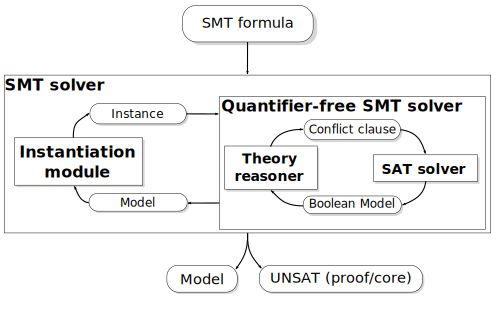
\includegraphics[height=0.5\textheight]{SMT1.pdf}}%
\only<2>{\includegraphics[height=0.5\textheight]{SMT2.pdf}}%
\only<3>{\includegraphics[height=0.5\textheight]{SMT3.pdf}}%
\only<4>{\includegraphics[height=0.5\textheight]{SMT4.pdf}}%
\only<5>{\includegraphics[height=0.5\textheight]{SMT5.pdf}}%
\only<6>{\includegraphics[height=0.5\textheight]{SMT6.pdf}}%
\only<7>{\includegraphics[height=0.5\textheight]{SMT7.pdf}}%
\only<8>{\includegraphics[height=0.5\textheight]{SMT8.pdf}}%
\only<9>{\includegraphics[height=0.5\textheight]{SMT9.pdf}}%
  \end{center}

\vspace*{-14pt}
\begin{footnotesize}
  Input: $a \leq b \wedge b \leq a + x \wedge x = 0 \wedge
  \big[ f(a) \neq f(b) \vee (q(a) \wedge \neg q(b + x)) \big]$

  \vspace*{2pt}
  \onslide<2->{
    To SAT solver: $p_{a \leq b} \wedge p_{b \leq a + x} \wedge p_{x = 0} \wedge
    \big[ \neg p_{f(a) = f(b)} \vee (p_{q(a)} \wedge \neg p_{q(b + x)}) \big]$}

  \vspace*{2pt}
  \onslide<3->{
    Boolean model: $p_{a \leq b}, p_{b \leq a + x}, p_{x = 0}, \neg p_{f(a) = f(b)}$}

  \vspace*{2pt}
  \onslide<4->{
    Theory reasoner: $a \leq b, b \leq a + x, x = 0, f(a) \neq f(b)$ unsatisfiable}

  \vspace*{2pt}
  \onslide<5->{New clause: $\neg p_{a \leq b} \vee \neg
    p_{b \leq a + x} \vee \neg p_{x = 0} \vee p_{f(a) = f(b)}$}

\end{footnotesize}

\end{frame}

%--------------------------------------------------------------------- SLIDE --
%------------------------------------------------------------------------------

\begin{frame}
  \frametitle{From propositional SAT to SMT: in practice}

  \begin{itemize}
  \item online decision procedures\\
    {\small theory checks propositional assignment on the fly}
  \item small explanations\\
    {\small unsat core of propositional assignment\\
    discard classes of propositional assignments (not one by one)}
  \item theory propagation\\
    {\small instead of guessing propositional variable
    assignments, SAT solver assigns theory-entailed literals}
  \item ackermannization, simplifications, and other magic
  \end{itemize}

\end{frame}

%--------------------------------------------------------------------- SLIDE --
%------------------------------------------------------------------------------

\begin{frame}
  \frametitle{Theory and quantifier reasoning}

  \begin{itemize}
  \item theory reasoning techniques specific to theories\dots
  \item \dots but (mostly) interact similarly with the SAT solver
  \item uninterpreted symbols and equality: congruence closure
  \item linear arithmetic: mostly simplex
  \item quantifiers: mostly instantiation
  \end{itemize}

  More details to come later (with proof production)

\end{frame}

%------------------------------------------------------------------- SECTION --
%------------------------------------------------------------------------------

\section{Proofs and SMT}

%--------------------------------------------------------------------- SLIDE --
%------------------------------------------------------------------------------

\begin{frame}
  \frametitle{From propositional SAT to SMT}

  \begin{center}
    \includegraphics[height=0.5\textheight]{SMT9.pdf}
  \end{center}

\vspace*{-14pt}
\begin{footnotesize}
  Input: $a \leq b \wedge b \leq a + x \wedge x = 0 \wedge
  \big[ f(a) \neq f(b) \vee (q(a) \wedge \neg q(b + x)) \big]$

  \vspace*{2pt}
  \onslide<2->{
    To SAT solver: $p_{a \leq b} \wedge p_{b \leq a + x} \wedge p_{x = 0} \wedge
    \big[ \neg p_{f(a) = f(b)} \vee (p_{q(a)} \wedge \neg p_{q(b + x)}) \big]$}

  \vspace*{2pt}
  \onslide<3->{New theory clause: $\neg p_{a \leq b} \vee \neg
    p_{b \leq a + x} \vee \neg p_{x = 0} \vee p_{f(a) = f(b)}$}

  \vspace*{2pt}
  \onslide<4->{New theory clause: $\neg p_{a \leq b} \vee \neg
    p_{b \leq a + x} \vee \neg p_{q(a)} \vee p_{q(b + x)}$}
\end{footnotesize}

\begin{block}{}
  SMT proof: interleaving of SAT proof and theory reasoning proof
\end{block}

\end{frame}
%% Challenge: collect enough information

%--------------------------------------------------------------------- SLIDE --
%------------------------------------------------------------------------------

\begin{frame}
  \frametitle{SMT in practice}

  \begin{itemize}
  \item online decision procedures\\
    {\small theory checks propositional assignment on the fly}\\
    {\it No influence on proof}
  \item small explanations\\
    {\small unsat core of propositional assignment\\
    discard classes of propositional assignments (not one by one)}\\
    {\it No influence on proof \small (small theory clauses)}
  \item theory propagation\\
    {\small instead of guessing propositional variable
    assignments, SAT solver assigns theory-entailed literals}\\
    {\it May need explanation (theory clause)}
  \item ackermannization, simplifications, and other magic\\
    {\it Sometimes cumbersome to prove}
  \end{itemize}

  \begin{block}{}
    Challenge: collect enough information
  \end{block}

\end{frame}

%--------------------------------------------------------------------- SLIDE --
%------------------------------------------------------------------------------

\begin{frame}
  \frametitle{Theory reasoning proofs}
  \framesubtitle{Congruence closure}
  Consider the terms: $a$, $b$, $c$, $f(a)$, $f(b)$

  \onslide<3->{And literals:} $\onslide<3->{a = c}\onslide<4->{, c = b}\onslide<6->{, f(a) \neq f(b)}$

\begin{minipage}{.4\textwidth}
  \begin{center}
\only<1>{\includegraphics[width=0.6\textwidth]{SMT-proof-CC0.pdf}}%
\only<2>{\includegraphics[width=0.6\textwidth]{SMT-proof-CC1.pdf}}%
\only<3>{\includegraphics[width=0.6\textwidth]{SMT-proof-CC2.pdf}}%
\only<4>{\includegraphics[width=0.6\textwidth]{SMT-proof-CC3.pdf}}%
\only<5>{\includegraphics[width=0.6\textwidth]{SMT-proof-CC4.pdf}}%
\only<6->{\includegraphics[width=0.6\textwidth]{SMT-proof-CC5.pdf}}%
  \end{center}
\end{minipage}%
\begin{minipage}{.55\textwidth}
\small
\begin{itemize}
\item<2-> each term in its equivalence class
\item<3-> equality $\longrightarrow$ class merge
\item<5-> congruence $\longrightarrow$ class merge
\item<6-> detect conflicts
\end{itemize}
\end{minipage}

\vspace*{10pt}
\onslide<7->{In practice: efficient (merge, congruence and conflict detection)}

\vspace*{10pt}
\onslide<8->{Theory reasoning proof, from graph:}
{\small
\begin{itemize}
\item<9-> conflict $f(a) \neq f(b)$ with an implied literal
\item<10-> entailed by congruence: $a \neq b \vee f(a) = f(b)$
\item<11-> and $a = b$ comes from transitivity: $a \neq c \vee c \neq b \vee a = b$
\item<12-> \emph{resolution} compute the theory clause: $a \neq c \vee c \neq b \vee f(a) = f(b)$
\end{itemize}}


\end{frame}

%--------------------------------------------------------------------- SLIDE --
%------------------------------------------------------------------------------

\begin{frame}
  \frametitle{Theory reasoning proofs}
  \framesubtitle{Combination of theories}

\onslide<1->{Theory reasoning proof, with combination of theories:}
{\small
\begin{itemize}
\item<1-> conflict $f(a) \neq f(b)$ with an implied literal
\item<2-> entailed by congruence: $a \neq b \vee f(a) = f(b)$
\item<3-> and $a = b$ comes from another theory clause: $\neg a \leq b \vee \neg b \leq a + x \vee x \neq 0 \vee a = b$
\item<4-> \emph{resolution} compute the theory clause: $\neg a \leq b \vee \neg b \leq a + x \vee x \neq 0 \vee f(a) = f(b)$
\end{itemize}}

\onslide<5->{
Over-simplification :
\begin{itemize}
\item delayed theory combination
\item model-based combination 
\end{itemize}}  

\end{frame}

%--------------------------------------------------------------------- SLIDE --
%------------------------------------------------------------------------------

\begin{frame}
  \frametitle{Theory reasoning proofs}
  \framesubtitle{Linear arithmetic}

  \begin{itemize}
  \item Many linear arithmetic decision procedures based on simplex
  \item Simplex detects inconsistency
  \item Farkas lemma can be used to provide certificate
  \end{itemize}

\begin{minipage}{.4\textwidth}
  \begin{center}
\only<1>{\includegraphics[width=0.8\textwidth]{SMT-proof-LRA0.pdf}}%
\only<2>{\includegraphics[width=0.8\textwidth]{SMT-proof-LRA1.pdf}}%
\only<3>{\includegraphics[width=0.8\textwidth]{SMT-proof-LRA2.pdf}}%
\only<4->{\includegraphics[width=0.8\textwidth]{SMT-proof-LRA3.pdf}}%
  \end{center}
\end{minipage}%
\begin{minipage}{.55\textwidth}
  \begin{itemize}
  \item \onslide<2->{$y>1$}\onslide<3->{, $x < 1$}\onslide<4->{, $y \leq x$}
  \item<5-> inconsistency\\
  \onslide<6->{
    \begin{tabular}{lc}
          & $x < 1$\\
      $+$ & $y \leq x$\\
      $-$ & $y>1$ \\
      \hline
      & $0 < 0$
    \end{tabular}}
  \item<7-> Clause: $\neg y>1 \vee \neg x < 1 \vee \neg y \leq x$
  \end{itemize}
\end{minipage}

\onslide<8->
{And also
\begin{itemize}
\item integers: branches, cuts
\item simplifications, bound propagations\dots
\end{itemize}
}

\end{frame}

%--------------------------------------------------------------------- SLIDE --
%------------------------------------------------------------------------------

\begin{frame}
  \frametitle{Quantifiers and proofs}

  \begin{itemize}
  \item
    Quantifiers mainly come from instantiation
  \item
    Proof is simply
    \begin{displaymath}
      \neg \forall x\, \varphi(x) \vee \varphi(t)
    \end{displaymath}
  \item
    $\forall x \varphi(x)$ is an abstract Boolean variable for the SAT solver
  \item
    Resolution, again
  \item
    Skolemization is a problem though
  \end{itemize}

\end{frame}

%% Prooving Theory Lemmas

%% Linear Arithmetic

%% Farkas' lemma


%% Integers



%--------------------------------------------------------------------- SLIDE --
%------------------------------------------------------------------------------

\begin{frame}
  \frametitle{Other theories}


Other theories
\begin{itemize}
\item arrays
\item inductive data types
\item bit-vectors
\item strings
\item non-linear arithmetic
\end{itemize}

\end{frame}

%------------------------------------------------------------------- SECTION --
%------------------------------------------------------------------------------

\section{Examples of SMT proofs}

%--------------------------------------------------------------------- SLIDE --
%------------------------------------------------------------------------------

\begin{frame}[fragile]
\frametitle{CVC4 proof (1/3)}

{\tiny
\begin{verbatim}
(check
(% a var_real
(% b var_real
(% x var_real
(% f (term (arrow Real Real))
(% q (term (arrow Real Bool))
(% @F1 (th_holds (<=_Real (a_var_real a) (a_var_real b)))
(% @F2 (th_holds (<=_Real (a_var_real b) (+_Real (a_var_real a) (a_var_real x))))
(% @F3 (th_holds (= Real (a_var_real x) (a_real 0/1)))
(% @F4 (th_holds (or (not (= Real (apply _ _ f (a_var_real a)) (apply _ _ f (a_var_real b)))) 
                     (and (= Bool (apply _ _ q (a_var_real a)) btrue)
                          (= Bool (apply _ _ q (+_Real (a_var_real b) (a_var_real x))) bfalse))))
(: (holds cln)

(decl_atom (<=_Real (a_var_real a) (a_var_real b)) (\ v1 (\ a1
(decl_atom (<=_Real (a_var_real b) (+_Real (a_var_real a) (a_var_real x))) (\ v2 (\ a2
(decl_atom (= Real (a_var_real x) (a_real 0/1)) (\ v3 (\ a3
(decl_atom (= Real (a_var_real a) (a_var_real b)) (\ v4 (\ a4
(decl_atom (= Real (apply _ _ f (a_var_real a)) (apply _ _ f (a_var_real b))) (\ v5 (\ a5
(decl_atom (= Bool (apply _ _ q (a_var_real a)) btrue) (\ v6 (\ a6
(decl_atom (= Bool (apply _ _ q (+_Real (a_var_real b) (a_var_real x))) bfalse) (\ v7 (\ a7
(decl_atom (<=_Real (a_var_real b) (a_var_real a)) (\ v8 (\ a8
(decl_atom (= Real (a_var_real a) (+_Real (a_var_real b) (a_var_real x))) (\ v9 (\ a9
(decl_atom (and (= Bool (apply _ _ q (a_var_real a)) btrue)
                (= Bool (apply _ _ q (+_Real (a_var_real b) (a_var_real x))) bfalse))
  (\ v10 (\ a10
\end{verbatim}
}
\end{frame}

\begin{frame}[fragile]
\frametitle{CVC4 proof (2/3)}

{\tiny
\begin{verbatim}

; CNFication
(satlem _ _ (asf _ _ _ a1 (\ l1 (clausify_false (contra _ @F1 l1)))) (\ C1 
(satlem _ _ (asf _ _ _ a2 (\ l2 (clausify_false (contra _ @F2 l2)))) (\ C2 
(satlem _ _ (asf _ _ _ a3 (\ l3 (clausify_false (contra _ @F3 l3)))) (\ C3
(satlem _ _ (ast _ _ _ a5 (\ l5 (asf _ _ _ a6 (\ l6 (clausify_false (contra _
  (and_elim_1 _ _ (or_elim_1 _ _ (not_not_intro _ l5) @F4)) l6)))))) (\ C4
(satlem _ _ (ast _ _ _ a5 (\ l5 (asf _ _ _ a7 (\ l7 (clausify_false (contra _
  (and_elim_2 _ _ (or_elim_1 _ _ (not_not_intro _ l5) @F4)) l7)))))) (\ C5

; Theory lemmas
; ~a4 ^ a1 ^ a8 => false
(satlem _ _ (asf _ _ _ a4 (\ l4 (ast _ _ _ a1 (\ l1 (ast _ _ _ a8 (\ l8
 (clausify_false (contra _ l1
 (or_elim_1 _ _ (not_not_intro _ (<=_to_>=_Real _ _ l8)) (not_=_to_>=_=<_Real _ _ l4))))))))))
 (\ C6 
; a2 ^ a3 ^ ~a8 => false
(satlem _ _ (ast _ _ _ a2 (\ l2 (ast _ _ _ a3 (\ l3 (asf _ _ _ a8 (\ l8 (clausify_false
 (poly_norm_>= _ _ _ (<=_to_>=_Real _ _ l2) (pn_- _ _ _ _ _ (pn_+ _ _ _ _ _
  (pn_var a) (pn_var x)) (pn_var b)) (\ pn2
 (poly_norm_= _ _ _ (symm _ _ _ l3) (pn_- _ _ _ _ _ (pn_const 0/1) (pn_var x)) (\ pn3
 (poly_norm_> _ _ _ (not_<=_to_>_Real _ _ l8) (pn_- _ _ _ _ _ (pn_var b) (pn_var a)) (\ pn8
 (lra_contra_> _ (lra_add_>_>= _ _ _ pn8 (lra_add_=_>= _ _ _ pn3 pn2)))))))))))))))) (\ C7
; a4 ^ ~a5 => false
(satlem _ _ (ast _ _ _ a4 (\ l4 (asf _ _ _ a5 (\ l5 (clausify_false
 (contra _ (cong _ _ _ _ _ _ (refl _ f) l4) l5)))))) (\ C8
\end{verbatim}
}
\end{frame}

\begin{frame}[fragile]
\frametitle{CVC4 proof (3/3)}

{\tiny
\begin{verbatim}

; a3 ^ a4 ^ ~a9 => false
(satlem _ _ (ast _ _ _ a3 (\ l3 (ast _ _ _ a4 (\ l4 (asf _ _ _ a9 (\ l9 (clausify_false
 (poly_norm_= _ _ _ (symm _ _ _ l3) (pn_- _ _ _ _ _ (pn_const 0/1) (pn_var x)) (\ pn3
 (poly_norm_= _ _ _ l4 (pn_- _ _ _ _ _ (pn_var a) (pn_var b)) (\ pn4
 (poly_norm_distinct _ _ _ l9 (pn_- _ _ _ _ _ (pn_+ _ _ _ _ _
  (pn_var b) (pn_var x)) (pn_var a)) (\ pn9
 (lra_contra_distinct _ (lra_add_=_distinct _ _ _
  (lra_add_=_= _ _ _ pn3 pn4) pn9))))))))))))))) (\ C9
; a9 ^ a6 ^ a7 => false
(satlem _ _ (ast _ _ _ a9 (\ l9 (ast _ _ _ a6 (\ l6 (ast _ _ _ a7 (\ l7 (clausify_false
 (contra _ (trans _ _ _ _ (trans _ _ _ _ (symm _ _ _ l6) (cong _ _ _ _ _ _
  (refl _ q) l9)) l7) b_true_not_false)))))))) (\ C10

; Resolution proof
(satlem_simplify _ _ _ (R _ _ (Q _ _ (Q _ _ C6 C1 v1) (Q _ _ (Q _ _ C7 C2 v2) C3 v3) v8)
(Q _ _ (Q _ _ (Q _ _ (Q _ _ (R _ _ C9 C10 v9) C3 v3) C4 v6) C5 v7) C8 v5) v4)
(\ x x)))))))))))))))))))))))))))))))))))))))))))))))))))))))))))))))
\end{verbatim}
}

\end{frame}

\begin{frame}[fragile]
\frametitle{veriT proof (1/2)}

{\tiny
\begin{verbatim}
(set .c1 (input :conclusion ((and (<= a b) (<= b (+ a x)) (= x 0)
                               (or (not (= (f b) (f a))) (and (q a) (not (q (+ b x)))))))))
(set .c2 (and :clauses (.c1) :conclusion ((<= a b))))
(set .c3 (and :clauses (.c1) :conclusion ((<= b (+ a x)))))
(set .c4 (and :clauses (.c1) :conclusion ((= x 0))))
(set .c5 (and :clauses (.c1) :conclusion
           ((or (not (= (f b) (f a))) (and (q a) (not (q (+ b x))))))))
(set .c6 (and_pos :conclusion ((not (and (q a) (not (q (+ b x))))) (q a))))
(set .c7 (and_pos :conclusion ((not (and (q a) (not (q (+ b x))))) (not (q (+ b x))))))
(set .c8 (or :clauses (.c5) :conclusion
           ((not (= (f b) (f a))) (and (q a) (not (q (+ b x)))))))
(set .c9 (eq_congruent :conclusion ((not (= a b)) (= (f b) (f a)))))
(set .c10 (la_disequality :conclusion ((or (= a b) (not (<= a b)) (not (<= b a))))))
(set .c11 (or :clauses (.c10) :conclusion ((= a b) (not (<= a b)) (not (<= b a)))))
(set .c12 (resolution :clauses (.c11 .c2) :conclusion ((= a b) (not (<= b a)))))
(set .c13 (la_generic :conclusion ((not (<= b (+ a x))) (<= b a) (not (= x 0)))))
(set .c14 (resolution :clauses (.c13 .c3 .c4) :conclusion ((<= b a))))
(set .c15 (resolution :clauses (.c12 .c14) :conclusion ((= a b))))
(set .c16 (resolution :clauses (.c9 .c15) :conclusion ((= (f b) (f a)))))
(set .c17 (resolution :clauses (.c8 .c16) :conclusion ((and (q a) (not (q (+ b x)))))))
(set .c18 (resolution :clauses (.c6 .c17) :conclusion ((q a))))
(set .c19 (resolution :clauses (.c7 .c17) :conclusion ((not (q (+ b x))))))
\end{verbatim}
}

\end{frame}

\begin{frame}[fragile]
\frametitle{veriT proof (2/2)}

{\tiny
\begin{verbatim}
(set .c20 (eq_congruent_pred :conclusion ((not (= a (+ b x))) (not (q a)) (q (+ b x)))))
(set .c21 (resolution :clauses (.c20 .c18 .c19) :conclusion ((not (= a (+ b x))))))
(set .c22 (la_disequality :conclusion
            ((or (= a (+ b x)) (not (<= a (+ b x))) (not (<= (+ b x) a))))))
(set .c23 (or :clauses (.c22) :conclusion
            ((= a (+ b x)) (not (<= a (+ b x))) (not (<= (+ b x) a)))))
(set .c24 (resolution :clauses (.c23 .c21) :conclusion
            ((not (<= a (+ b x))) (not (<= (+ b x) a)))))
(set .c25 (eq_congruent_pred :conclusion
            ((not (= a b)) (not (= (+ a x) (+ b x))) (<= a (+ b x)) (not (<= b (+ a x))))))
(set .c26 (eq_congruent :conclusion ((not (= a b)) (not (= x x)) (= (+ a x) (+ b x)))))
(set .c27 (eq_reflexive :conclusion ((= x x))))
(set .c28 (resolution :clauses (.c26 .c27) :conclusion ((not (= a b)) (= (+ a x) (+ b x)))))
(set .c29 (resolution :clauses (.c25 .c28) :conclusion
            ((not (= a b)) (<= a (+ b x)) (not (<= b (+ a x))))))
(set .c30 (resolution :clauses (.c29 .c3 .c15) :conclusion ((<= a (+ b x)))))
(set .c31 (resolution :clauses (.c24 .c30) :conclusion ((not (<= (+ b x) a)))))
(set .c32 (la_generic :conclusion ((<= (+ b x) a) (not (= a b)) (not (= x 0)))))
(set .c33 (resolution :clauses (.c32 .c4 .c15 .c31) :conclusion ()))
\end{verbatim}
}

\end{frame}

\begin{frame}[fragile]
\frametitle{z3 proof (1/2)}

{\tiny
\begin{verbatim}
(let (($x82 (q b)) (?x49 (* (- 1.0) b)) (?x50 (+ a ?x49))
      ($x51 (<= ?x50 0.0)) (?x35 (f b)) (?x34 (f a))
      ($x36 (= ?x34 ?x35)) ($x37 (not $x36))
      ($x43 (or $x37 (and (q a) (not (q (+ b x))))))
      ($x33 (= x 0.0)) (?x57 (+ a ?x49 x)) ($x56 (>= ?x57 0.0))
      ($x44 (and (<= a b) (<= b (+ a x)) $x33 $x43))
      (@x60 (monotonicity (rewrite (= (<= a b) $x51))
                          (rewrite (= (<= b (+ a x)) $x56))
                          (= $x44 (and $x51 $x56 $x33 $x43))))
      (@x61 (mp (asserted $x44) @x60 (and $x51 $x56 $x33 $x43)))
      (@x62 (and-elim @x61 $x51)) ($x71 (>= ?x50 0.0)))
(let ((@x70 (trans (monotonicity (and-elim @x61 $x33) (= ?x57 (+ a ?x49 0.0)))
                   (rewrite (= (+ a ?x49 0.0) ?x50)) (= ?x57 ?x50))))
(let ((@x74 (mp (and-elim @x61 $x56) (monotonicity @x70 (= $x56 $x71)) $x71)))
(let ((@x121 (monotonicity (symm ((_ th-lemma arith eq-propagate 1 1) @x74 @x62 (= a b)) (= b a))
                           (= $x82 (q a)))))
(let (($x38 (q a)) ($x96 (or (not $x38) $x82)) ($x97 (not $x96)))
(let ((@x115 (monotonicity (symm ((_ th-lemma arith eq-propagate 1 1) @x74 @x62 (= a b)) (= b a))
                           (= ?x35 ?x34))))
(let (($x100 (or $x37 $x97)))
(let ((@x102 (monotonicity (rewrite (= (and $x38 (not $x82)) $x97))
                           (= (or $x37 (and $x38 (not $x82))) $x100))))
(let (($x85 (not $x82)))
(let (($x88 (and $x38 $x85)))
(let (($x91 (or $x37 $x88)))
(let ((@x81 (trans (monotonicity (and-elim @x61 $x33) (= (+ b x) (+ b 0.0)))
                   (rewrite (= (+ b 0.0) b)) (= (+ b x) b))))
(let ((@x87 (monotonicity (monotonicity @x81 (= (q (+ b x)) $x82)) (= (not (q (+ b x))) $x85))))
\end{verbatim}
}

\end{frame}

\begin{frame}[fragile]
\frametitle{z3 proof (2/2)}

{\tiny
\begin{verbatim}
(let ((@x93 (monotonicity (monotonicity @x87 (= (and $x38 (not (q (+ b x)))) $x88))
                          (= $x43 $x91))))
(let ((@x103 (mp (mp (and-elim @x61 $x43) @x93 $x91) @x102 $x100)))
(let ((@x119 (unit-resolution (def-axiom (or $x96 $x38))
                              (unit-resolution @x103 (symm @x115 $x36) $x97) $x38)))
(let ((@x118 (unit-resolution (def-axiom (or $x96 $x85))
                              (unit-resolution @x103 (symm @x115 $x36) $x97) $x85)))
(unit-resolution @x118 (mp @x119 (symm @x121 (= $x38 $x82)) $x82) false)))))))))))))))))
\end{verbatim}
}

\end{frame}

\section{Applications and Challenges}

\begin{frame}\frametitle{Applications}

\begin{block}{Current Applications}
\begin{itemize}
\item Proof reconstruction within skeptical proof assistants
\footnote{
\tiny Keller. {\bf A Matter of Trust: Skeptical Communication Between Coq and
  External Provers}, PhD Thesis, Ecole Polytechnique, 2013.}$^{,}$
\footnote{
\tiny Armand, Faure, Gr{\'e}goire, Keller, Thery, Werner. {\bf A Modular
  Integration of SAT/SMT Solvers to Coq through Proof Witnesses}, CPP '11.}$^{,}$
\footnote{
\tiny B{\"o}hme. {\bf Proof Reconstruction for Z3 in Isabelle/HOL}, SMT'09.}

\item Interpolant generation
\footnote{
\tiny Reynolds, Tinelli, Hadarean. 
{\bf Certified Interpolant Generation for EUF}, SMT '11.}$^{,}$
\footnote{
\tiny Hofferek, Gupta, K\"{o}nighofer, Jiang, Bloem.
{\bf Synthesizing Multiple Boolean Functions using Interpolation on a Single
  Proof}, FMCAD '13.}$^{,}$
\footnote{
\tiny McMillan.
{\bf Interpolants from Z3 Proofs}, FMCAD '11.}

\item Unsat core computation
\footnote{\tiny D\'{e}harbe, Fontaine, Guyot, Voisin.
{\bf SMT Solvers for Rodin}, Abstract State Machines '12.}

\end{itemize}
\end{block}
\end{frame}

\begin{frame}\frametitle{Challenges}

\begin{block}{Challenges}
\begin{itemize}
\item Challenge to collect and store proof information efficiently
\item Producing proofs for sophisticated preprocessing techniques
\item Producing proofs for modules that use external tools
\item Standardizing a proof format
\end{itemize}
\end{block}
\end{frame}

\begin{frame}
\frametitle{Lean Theorem Prover}
  \begin{itemize}
    \item New theorem prover started by L. de Moura and Soonho Kong.
    \item {\small Contributors: Jeremy Avigad, Cody Roux, Floris van Doorn,\\ Parikshit Khanna}
    \item {\small Many thanks to: Georges Gonthier, Nikhil Swamy, Vladimir Voevodsky}
  \end{itemize}
  \vspace*{12pt}
  \begin{itemize}
    \item Open source (Apache 2.0), {\small \url{https://github.com/leanprover/lean}}
    \item {\color{red} can be used as an automatic prover (SMT), and as a proof assistant}
    \item Based on {\color{red} Type Theory}, and incorporates ideas of many other systems:\\
        Agda, Coq, HOL-Light, Isabelle, PVS, ...
  \end{itemize}
\end{frame}

\begin{frame}
\frametitle{Lean: Two Layers Architecture}
  \begin{itemize}
     \item {\color{red} First layer}: type checker, APIs for creating terms, environment, ...
     \item Configuration options: e.g., impredicative Prop, proof irrelevance, ...
     \item Universe polymorphism.
     \item 5k lines of C++ code.
  \end{itemize}
  \vspace*{12pt}
  \begin{itemize}
     \item {\color{red} Second layer}: additional (trusted) components.
     \item Example: inductive datatypes (extra 500 lines of code).
     \item We currently support two flavors/instances: {\color{red} Standard} and {\color{red} HoTT}.
  \end{itemize}
\end{frame}

\begin{frame}
\frametitle{Lean: As a Library}
  \begin{itemize}
     \item Meant to be used as a {\color{red} standalone system} and as a {\color{red} software library}.
     \item Extensive API and can be easily embedded in other systems.
     \item SMT solvers can use the Lean API to create proof terms that can be independently checked.
     \item APIs in C++, Lua (and Python coming soon).
  \end{itemize}
\end{frame}

\begin{frame}
\frametitle{Lean: Proofs}
  \begin{itemize}
  \item More expressive language for encoding proofs provides several
advantages.
  \item {\color{red} We can easily add new ``proof rules'' without
modifying the proof checker} (i.e., type checker).
  \item Proof rules such as {\color{red} mp} and {\color{red} monotonicity} used in Z3 are just theorems in Lean.
  \end{itemize}
\end{frame}

\begin{frame}[fragile]
\frametitle{Lean: Automation}
  \begin{itemize}
  \item First, define theory, then prove theorems/properties, then implement automation.
  \item Example: suppose we are implementing a procedure for Presburger Arithmetic.
  \end{itemize}

{\tiny
\begin{verbatim}
       theorem add_comm (n m:nat) : n + m = m + n
       := induction_on m
         (trans (add_zero_right _) (symm (add_zero_left _)))
         (take k IH,
            calc n + succ k = succ (n+k) : add_succ_right _ _
                        ... = succ (k + n) : {IH}
                        ... = succ k + n : symm (add_succ_left _ _))
\end{verbatim}
}
\end{frame}

\begin{frame}[fragile]
\frametitle{Lean: Automation}
  \begin{itemize}
  \item Pre-processing steps such as Skolemization can be supported in
a similar way.
  \end{itemize}

{\tiny
\begin{verbatim}
  theorem skolem_th {A : Type} {B : A -> Type} {P : forall x : A, B x -> Bool} :
                (forall x, exists y, P x y) = (exists f, (forall x, P x (f x)))
   := iff_intro
       (assume H : (forall x, exists y, P x y), axiom_of_choice H)
       (assume H : (exists f, (forall x, P x (f x))),
          take x, obtain (fw : forall x, B x) (Hw : forall x, P x (fw x)), from H,
            exists_intro (fw x) (Hw x))
\end{verbatim}
}
\end{frame}

\begin{frame}[fragile]
\frametitle{Lean: Pre-processing}
  \begin{itemize}
     \item The pre-processing ``issue'' is addressed by providing a {\color{red} generic rewriting
engine} that can use any previously proved theorems.
     \item The engine accepts two kinds of theorems: {\color{red} congruence theorems} and {\color{red} (conditional)
equations}.
     \item It also supports a $\lambda$-Prolog like engine.
  \end{itemize}

{\tiny
\begin{verbatim}
           theorem forall_or_distributel {A : Type} (p : Bool) (q : A -> Bool)
                   : (forall x, q x \/ p) = ((forall x, q x) \/ p)
           theorem forall_or_distributer {A : Type} (p : Bool) (q : A -> Bool)
                   : (forall x, p \/ q x) = (p \/ forall x, q x)
\end{verbatim}
}

\end{frame}


\end{document}
